 % -*- root: ../medieninformatik-arbeit.tex -*-
\documentclass[../medieninformatik-arbeit.tex]{subfiles}
\begin{document}
\section{Prototype Design}
\label{ch:proto}
This chapter presents the process of developing the designs for the activity sculpture and the web configurator. In the first section the requirements for the activity sculpture are presented with four different prototypes that attempt to fulfill the requirements. Finally the validation process for the sculpture to be designed will be discussed. The second section is devoted to the design process of the customization system. This comprehends not only the user interface but also the user experience while operating the system. After a process where three different concepts were ideated, through the validation of the design the final prototype is chosen. 

\subsection{Activity Sculpture Design}
The activity sculpture and the configurator are strongly interconnected as depending of the sculpture design, the sculpture will influence the quantity of controls to be taken into consideration for the design of the configurator. This traduces in users having greater or lesser freedom for manipulating the the sculpture. As we discussed in section \ref{sec:activitysculptures}, activity sculptures portray different attributes inherit from their physical nature. This is why a different approach for designing physical data visualizations is needed. For this purpose the design taxonomy proposed by Vande Moere et al. \cite{vande2009analyzing} was used as a guide to better categorize the qualities of the developed designs. This taxonomy has two dimensions which describe the design space of activity sculptures: \textit{representational fidelity} and \textit{narrative formulation}. 

\textbf{The representational fidelity} attempts to explain the decisions made for the embodiment of the data in form. This includes the chosen metaphor for mapping the data to the object and the resulting metaphorical distance. This is the level of abstraction used to represent the data through the metaphor. In order to better explain the abstraction level Vande Moere's taxonomy uses concepts from semiotic studies. According to C.K. Ogden et al. \cite{ogden1946meaning} semiotic signs can be explained through three major concepts: the signified, the signifier and the sense. The signified is an object that represents a physical thing or and idea. The signified is represented by the signifier who tries to bring the same experience an observer would have with the signified. The sense is the experience brought by the signified. Furthermore signs can be categorized into iconic, indexical and symbolic. Iconic representation occurs when the signifier resembles the signified, like a picture or a diagram. Activity sculptures are iconic when they resemble the metaphor they are interpreting. Examples of this could be the heartrate extruded graph sculpture discussed in section \ref{sub:sweatatoms} or the MakerVis visualizations in \ref{fig:makervis-config}. An indexical sign has a sensory feature that correlates directly to the signified. The signifier points to the signified through an actual connection, like dark clouds point to forthcoming rain or smoke points to fire. Activity sculptures can be classified as indexical when they make use of a property directly related to the data. An example of such a sculpture would be the SweatAtoms frog in section \ref{sub:sweatatoms} or the . The most complex kind of sing is the symbol, as it does not bear any resemblance to the signified. The relationship between the signified and the signifier has to be taught by convention in order to be understood. Activity sculptures making use of symbolic representation are the hardest to understand as the relationship to the data has to be learned as it is not apparently displayed. Example of symbolic sculptures would be the landscapes in the Mental Fabrications project discussed in section \ref{sub:mentalfabrications}. Through the definition of iconic, indexical and symbolic representation we can derive their metaphorical distance resulting in indexical having the closest distance, symbolic the farthest and iconic a medium distance \cite{swaminathan2014supporting}. 

\textbf{The narrative formulation} of activity sculptures is a product of the physical form and the affordance of the object which influences the user's ability to discover information through interaction and perception. This quality is strongly interconnected to the representational fidelity as the level of abstraction in which the data is presented will form the properties through which the sculpture communicates. As discussed in section \ref{sec:activitysculptures} the affordance of an object describes to the viewer the object's potential to perform an action. The level of abstraction of the sculpture will influence how inviting the object is to the viewer depending on the user's level of familiarity with the metaphor used. 

Computer aided design systems offer almost endless possibilities in the design of activity sculptures, allowing designers to create complex structure designs that would be almost impossible to conceive with manual methods it. Even though this might be the case in the digital realm, translating the virtual object into a physical object may be still a challenge. An important aspect to be considered while developing activity sculptures is the manufacturability of the sculpture \ \cite{swaminathan2014supporting}. 3D printing machines still are challenged by certain types of structures depending on the technology that is being used to manufacture (granular vs extrusion methods). Therefore it is important to take into account how challenging the manufacturability of the sculpture will be.

The aforementioned design considerations of activity sculptures were considered for specifiying the requirements for the activity sculptures. They were formulated as follows. 

\begin{itemize}
	\item The sculpture has to be aesthetically appealing to users
	\item Motivate users to self reflection
	\item Because of the wide range of activity data types obtained through the fitness tracker, the sculpture has to be able to visualize as many variables as possible
	\item In order to provide users a relatively high level of freedom while customizing the sculpture, the sculpture has to offer multiple configuration options
	\item The sculpture has to be extended to new interaction forms
	\item The sculpture has to be 3D printable by current 3D printing technologies
\end{itemize}

With the defined requirements the author formulated four designs exploring different possible approaches. Due to space and layout considerations, the sketches drawn for the prototypes will not be displayed in this chapter, only fragments. The sketches for all prototypes were placed in their entirety in the appendix of this work. For the sculpture prototypes sketches please refer to section \ref{App:proto-sculptures}, for configurator prototypes sketches refer to section \ref{App:proto-config}.

\subsubsection{3D Graph}
The first prototype is based on a line chart but augmented to describe more data variables. The idea was inspired by multiple exposure images of Olympic athletes in the middle of their performance. The multi exposure technique allows photographers to take a snapshot of the athlete at a specific point in time. The resulting image shows a group of athletes in different positions completing a cycle of a movement (see figure \ref{fig:multiexposure}). The concept of presenting snapshots of the athlete's position over time is actually a parallel concept to standard charts and charts where the value of a variable is presented at a specific point in time. Only transferring the line-chart to physical space would have been not appealing enough and very limited as it would have been only possible to visualize one variable over time. The first modification made in order to improve the aesthetic of the sculpture was to give the chart-line volume and a triangulated or low polygon count (lowpoly) aesthetic, two properties that can be explored thanks to physical space. With this modification the sculpture gained the ability to visualize one more variable. The first variable influences the height changes in the Y axis of the chart-line over time and by adding the volume to the line we can change the radius of the line according to the value changes of the variable over time. 

\begin{figure}[ht]
\captionsetup{width=0.8\textwidth}
\begin{center}
  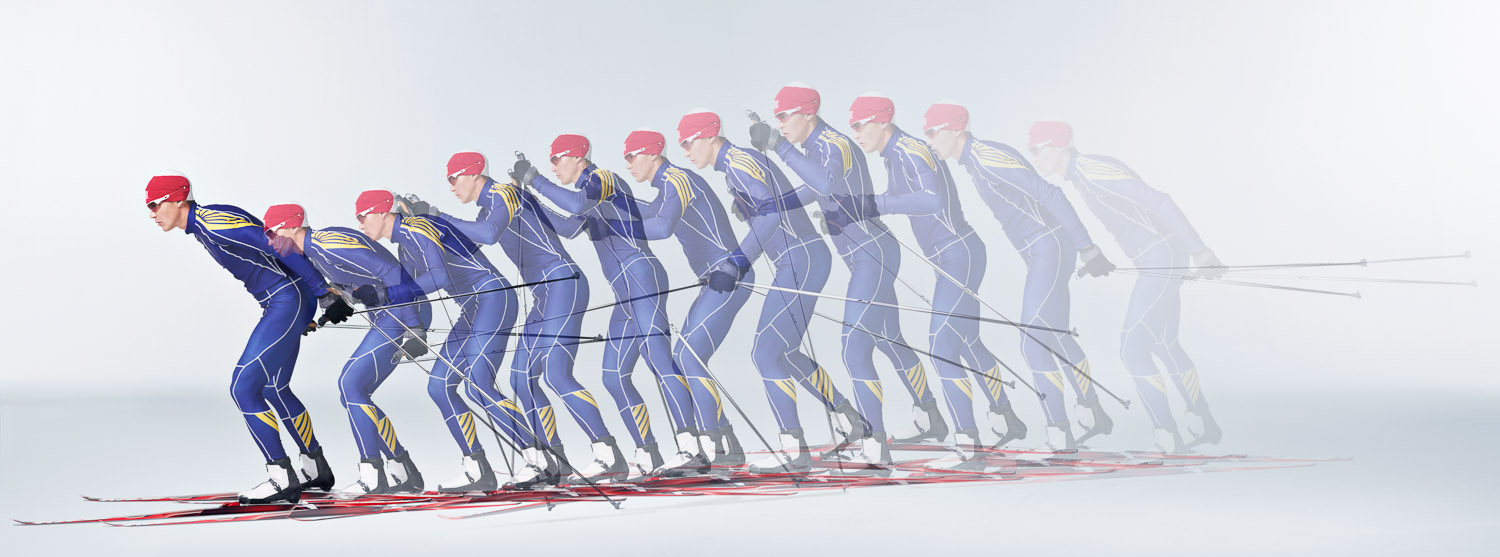
\includegraphics[width=0.8\textwidth]{Prototype/img/multiexposure}
  \caption{Athlete's movements captured in a multiple exposure image \cite{multiexposure}}
\label{fig:multiexposure}
\end{center}
\end{figure}

Up until this point the 3D graph would look as shown in figure \ref{fig:3DgraphDetail}. It visualizes up to 2 variables over time. Even though the data is being visualized as an abstract triangulated body with hight and radius changes the sculpture could take advantage of the depth dimension not only to display volume but to steer the body in this dimension. Through this realization, the 3D graph now can map 3 variables. To further enhance the aesthetic of the sculpture the concept of the athlete's snapshot in specific points of time was further explored. For this a set of avatars performing different sports were developed. These avatars would intersect the graph body in specified intervals by the user. By adding different avatars performing a variety of sports users can choose the avatar that represents best the sport or activity the user did to generate the data. The sculpture could be expanded to support different decoration styles. For example apart from the triangulated look of the graph body, other visualization styles like a wire-frame option or a smoothed could be offered. 
As shown in figure \ref{fig:3DgraphDetail}, the whole structure looks as if it would float in the air with the help of a support structure, which could be manufactured separately from transparent acrylic  so that they fade away centering the attention in the sculpture. This support structure would be inserted into a wooden or acrylic plate. The author explored the idea of engraving a summary of the data the sculpture represents. In this way users have both the abstract visualization and the actual data in the same place close enough to analyze. This might be useful while showing it to others, as it can help them better grasp what the sculpture represents. By adding a plate to the sculpture we open a new set of configuration possibilities for users to edit in the configurator. 

The 3D graph embodies activity data through iconic and indexical representations. Indexical because as stated before, the concept emerged from an expanded line-chart an the graph body points to the path line-chart would have but abstracted and stylized and with the avatars in different positions point to movement in activity. The avatars are a strong icon of a human body in motion. The 3D graph shows a somewhat short metaphorical distance as the sculpture points strongly to  the line-chart metaphor used to embody the data. In the narrative formulation of the sculpture again the chart-graph resemblance and the plate tell the user this object is to be analyzed or at least admired as the plate does not allow grabbing the sculpture. Self reflection is highly encouraged as the metaphor motivates comparison of values over time. 

\begin{figure}[h]
\captionsetup{width=0.8\textwidth}
\begin{center}
  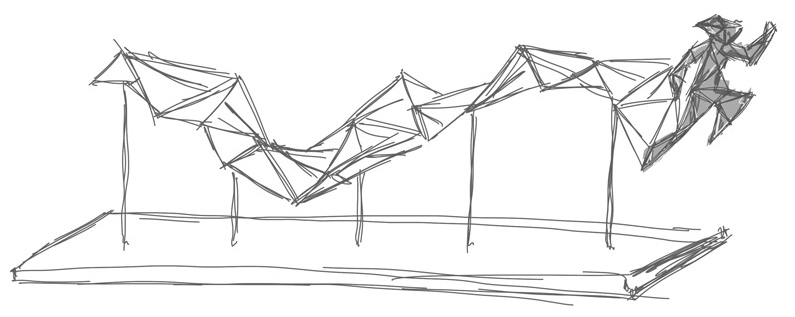
\includegraphics[width=0.8\textwidth]{Prototype/img/3DGraph_detail}
  \caption{3D Graph sketch}
\label{fig:3DgraphDetail}
\end{center}
\end{figure}

In summary, the 3D Graph prototype is a highly aesthetic activity sculpture that is also functional as the both the sculpture and the data could be analyzed in the same object. The sculpture can visualize data generated on a large time span. it has a rather low capability of mapping several variables because of the constraints of the line-chart metaphor. This could be improved by adding more graph bodies representing each 3 variables over time. The 3D graph offers a wide range of configuration options that would make it a rather interesting object to customize in the configurator. The manufacturability of the sculpture is attainable but also complicated as the sculpture, the plate and the supporting elements have to be fabricated not to mention the engravings on the plate. 

\subsubsection{Activity Landscape}
The activity landscape is an activity sculpture that embodies data gathered throughout a day by utilizing the data to generate a terrain (see figure \ref{fig:activitylandscape}. The concept of this sculpture came from the idea of generating a ground path from the GPS location points recollected while a user was jogging or riding his bike. During the workout other activity information like heart rate or elevation change is also recorded and would be then mapped to the GPS location points. The user would then select in the configurator which variables he wants to map to different aspects of the terrain and experiment with different variables for terrain elevation or for the radius of hills for instance. The activity landscape would also feature a plate for showcasing the sculpture. This plate as in the 3D Graph would feature engraved information about the workout like variables visualized, duration of the workout and calories burned. Because the terrain is based mostly on GPS information, the plate could also have a picture or engraving of a map where the workout was performed. As seen in section \ref{sub:sweatatoms} where some users stacked sculptures to form a bigger sculpture, several activity landscapes could be printed to form a bigger landscape. This could be used to motivate users to explore new parts of their city, it would be interesting to see how the landscape would look like after a year running or biking. This concept could also be applied to users who maybe travel constantly or like to ride their bikes in national parks around the world. After each travel they could bring the memories of their adventure in an activity landscape and put them together at their homes. 

\begin{figure}[h]
\centering
\begin{minipage}{.45\textwidth}
\centering
	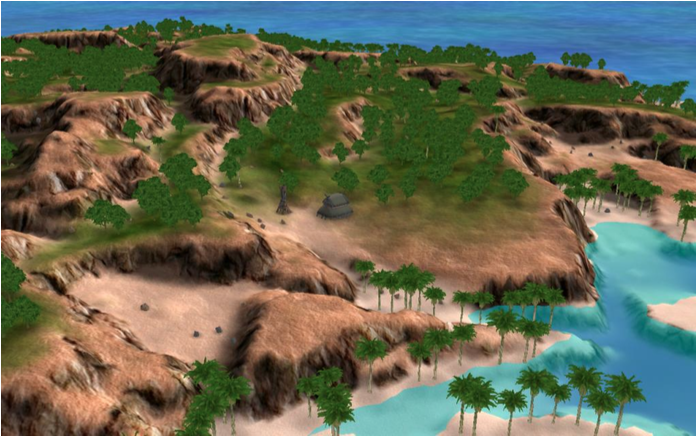
\includegraphics[width=\linewidth]{Prototype/img/terrain}
	\caption{Procedurally generated landscape \ \cite{olsen2004realtime}}
	\label{fig:proceduralterr}
\end{minipage}
\begin{minipage}{.45\textwidth}
\centering
  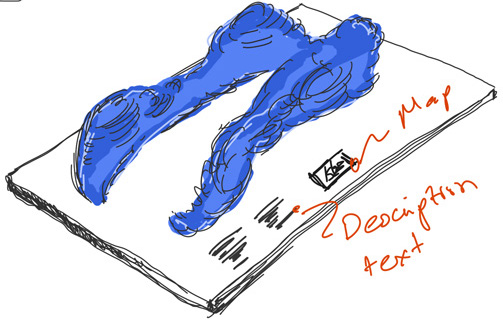
\includegraphics[width=0.88\linewidth]{Prototype/img/ActivityLandscape_detail}
  \caption{Activity Landscape sketch}
  \label{fig:activitylandscape}
\end{minipage}
\end{figure}

The inspiration for this sculpture was taken from the game development field where, with advances in processing power terrains for games are not being loaded from 3D model assets bur rather generated in real time even with complex erosion simulations \cite{olsen2004realtime} (see figure \ref{fig:proceduralterr}). After looking at several generated terrains the concept of utilizing activity data to manipulate the generation of a terrain emerged. It would be interesting to see the configuration process as every time the user selects a different variable to manipulate the terrain, new sceneries would emerge.

The activity landscape embodies the activity data through iconic representation as the terrain resembles some characteristics of the data like elevation and geographical position for example thus exhibiting a medium metaphorical distance. The level of affordance is low as it only invites the user to contemplate and self reflect. 

To summarize, the activity terrain provides an interesting approach to activity visualization and maybe also to procedural terrain generation in games. The level of customization in the configurator is high. It has to be clarified that the complexity of designing terrain generation algorithms was not studied in depth by the author, therefore it remains unknown how many variables are possible to visualize through the terrain. The added plate with the map can give users a stronger sense of belonging to their city. The idea of a personalized souvenir from adventure rides would be also interesting to explore. The sculpture does not exhibit any properties that could prove to be difficult to manufacture. Same as the with the 3D Graph the plate could only make the fabrication process somewhat longer.  

\subsubsection{Activity Flora}
The activity flora is an activity sculpture that utilizes activity data as input parameters for the generation of a sculpture resembling a leaf. The concept for this prototype is to take the data generated in a single day or during a single workout and materialize it in a leaf like structure. In the sketch showed in figure \ref{fig:activityflora} activity data variables can be mapped to properties of the leaf. For example the size of the leaf could be affected by the traversed distance during that day, the contour shape could be mapped to elevation changes. The main branch in the middle of the leaf could be manipulated by the velocity changes, furthermore the characteristic branch structure inside the leaf could be influenced by the average heartrate value (see figure \ref{fig:activityflora}). For the inner structure of the leave a generative system could be implemented to simulate better the leaf structure. In the configurator users could select which variable to map to each leaf generation parameter to generate a series of leafs. The customization possibilities could be further expanded with the addition of leaf tails and material options. To further explore the concept of grouping sculptures, a sketch with a stand that holds several leafs was drawn like a very stylized flower pot. The leaf stand or pot would also be able to be customizable in the configurator.  

\begin{figure}[h]
\captionsetup{width=0.6\textwidth}
\begin{center}
  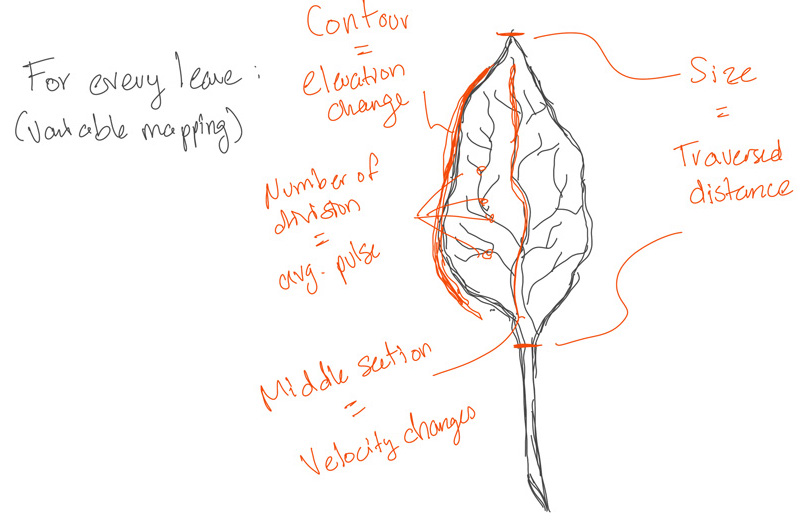
\includegraphics[width=0.6\textwidth]{Prototype/img/ActivityFlora_detail}
  \caption{Activity Flora sketch}
\label{fig:activityflora}
\end{center}
\end{figure}

The idea was inspired by the works of New York based generative design studio Nervous System \cite{nervousStudio} who since 2007 have been pioneering the design of generative objects for 3D printing. The majority of their designs is based in the simulation of natural structures or patterns through algorithms (see figure \ref{fig:nervous}). The concept of generating an object from activity data with an aesthetic inspired by nature was very appealing to the author. It would be interesting to see how users engage and perceive an object that was generated by their own activity but that also looks like something that use to live, like a petrified leaf. Maybe in the future when 3D printing is also possible to do with biologic materials some kind of bacteria culture could be utilized to print the leaf and make it a living object for real. 

\begin{figure}[h]
\captionsetup{width=0.7\textwidth}
\begin{center}
  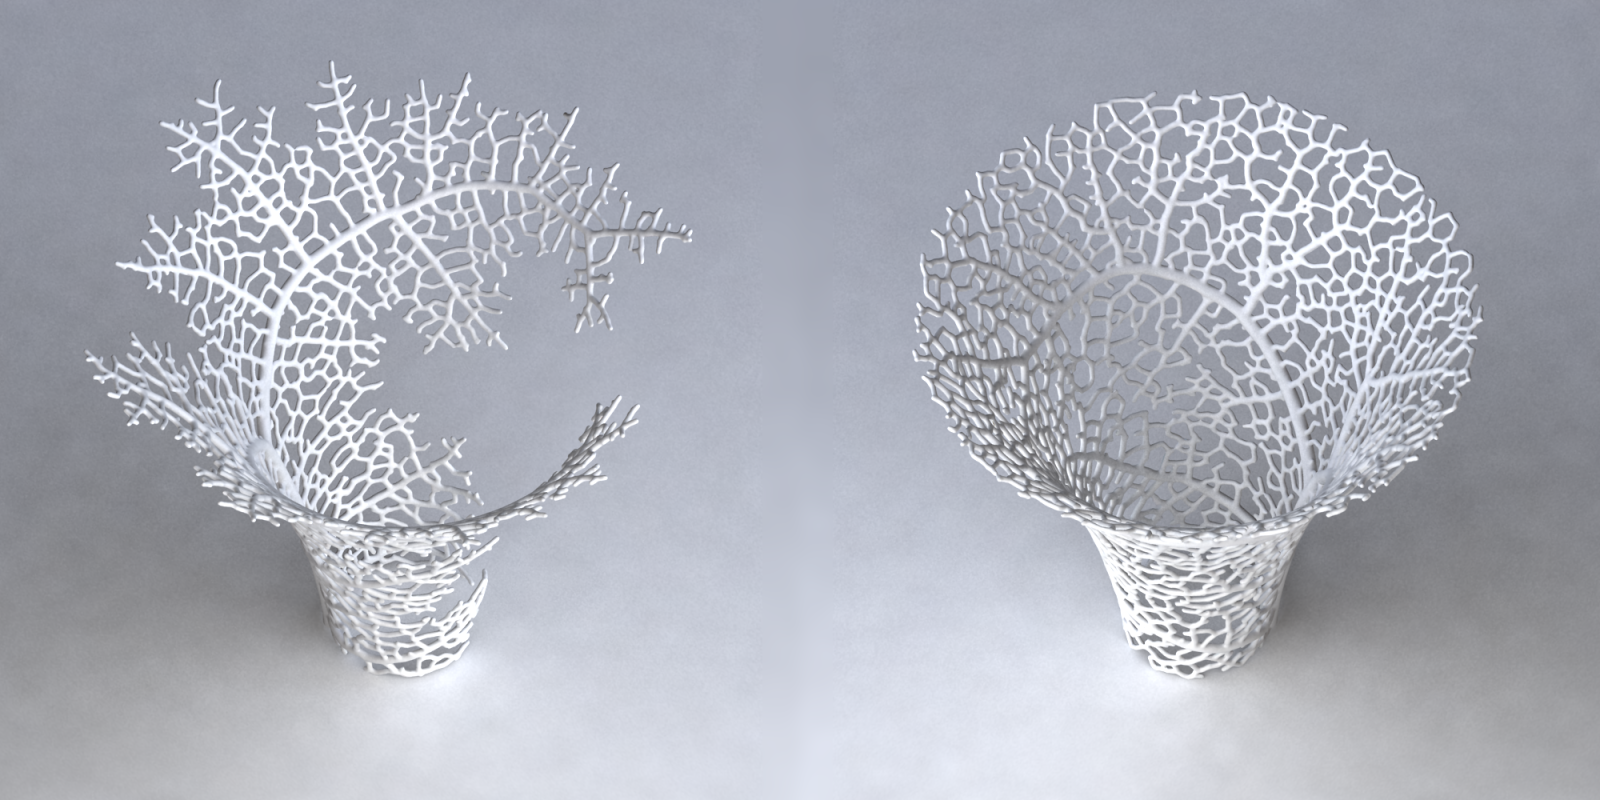
\includegraphics[width=0.7\textwidth]{Prototype/img/nervous}
  \caption{Sculptures made with generative algorithms based on hyphae growth as seen on leave and coral structures \cite{nervousHyphae}}
\label{fig:nervous}
\end{center}
\end{figure}

The activity flora embodies the data mostly iconic representation as the sculpture resembles a leaf but some information is abstracted completely because of the generative system resulting in a medium high metaphorical distance. The leaf prototype invites the user to contemplate the sculpture and due to the metaphor of the leaf self reflection will be harder for the viewer as the data is mapped not entirely to the sculpture but also to the system generating the leaf's structure.

To conclude this prototype, the activity leaf showcases a mixed approach to activity sculpture design, mapping some variables to physical properties of the leaf and using activity data as input for a generative system. The configuration possibilities are rather scarce and focus more on secondary elements of the sculpture like the stand or the leaf tail. The concept of metaphorically giving an object natural characteristics would be interesting to explore in the context of activity sculptures.

\subsubsection{Activity Vase}
\label{sub:activtyvase}
The last developed prototype is the activity vase, a sculpture where the structure is conformed of a stacked radial chart with smoothly connected axes. Every stacked radial chart represents a day's worth of activity. The user can choose in the configurator how many variables he wants to add to the vase by populating the radial chart. The height of the vase would be then configured by choosing the time span to be visualized which translates in the number of stacked radial charts (see figure \ref{fig:activityvase}). In this way the configurator can offer the user different outputs from one sculpture. Users could gain different usages of the sculpture depending on the visualized time span. For short time spans the sculpture could be expanded or adapted to be used as earrings or as a key-chain, longer time spans could be then used to make a pen holder or even a mug. Users could print each day the visualized data and maybe stacked them in a pole. As the sculpture better visualizes larger time spans from at least a day to weeks or months a sculpture representing two months in a year could be visualized, for example at the beginning and at the end of an intense workout plan an inner solid sculpture would represent the first month and an outer sculpture enclosing the first would represent the last month as it is expected that the activity performed will contain higher values in some variables, as the user reaches longer distances in their trainings for example. The sculpture could be further customized in the configurator through 3D printing material options and maybe even a simple plate where the labels of the variables are engraved. 

The concept of the activity vase was inspired by a 3D printed sculpture that maps two or more facial profiles to the sides of a vase and then unites them through extrusion. The final product is called Fhaz (see figure \ref{fig:fhaz}), which is basically an expansion of Rubin's vase \cite{rubin1921visuell} to visualize more than two profiles in a 3D printed object. In order to transfer the concept of Rubin's vase to an activity sculpture the idea of utilizing a stacked radial chart proved to be a suitable solution.

Using Vande Moere's taxonomy, the activity vase embodies the activity data through a symbolic representation as the visualization has no resemblance to the metaphor. As the abstraction of the represented data in the sculpture is high the metaphorical distance is also high. The activity vase offers viewers the freedom to explore the sculpture through touch and self-reflection because of the viewer's low familiarity with the object. The narrative has to be figured out through exploration and interaction with the object.

The activity vase is a very flexible sculpture in terms of data mapping. Through the radial chart metaphor the visualized amount of variables is only limited by the users decisions in the configurator. Due to its abstract representation the sculpture could be adapted to be used as everyday accessories and is not only limited to standing in a shelf. The configurability of the sculpture is not very high but this could be addressed through the addition of different rendering styles to the configurator like wire-frame visualization for instance. The manufacturability of the sculpture is attainable as the solid structure of the vase does not challenge current fabrication methods. 


\begin{figure}[h]
\centering
\begin{minipage}{.45\textwidth}
\centering
	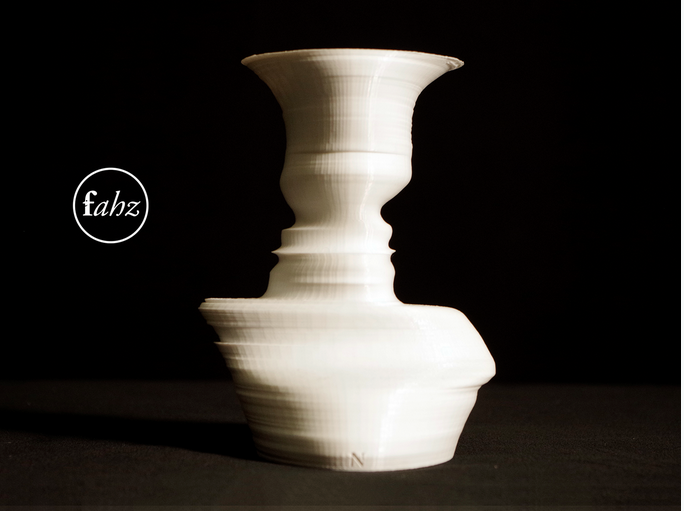
\includegraphics[width=\linewidth]{Prototype/img/fhaz}
	\caption{Fhaz: Procedurally generated vase based on facial profiles\ \cite{fahz}}
	\label{fig:fhaz}
\end{minipage}
\begin{minipage}{.45\textwidth}
\centering
  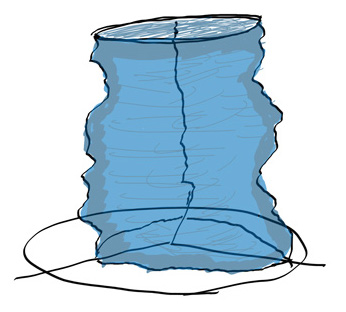
\includegraphics[width=0.75\linewidth]{Prototype/img/ActivityVase_detail}
  \caption{Activity Vase sketch}
  \label{fig:activityvase}
\end{minipage}
\end{figure}

\subsubsection{Prototype Validation}
After an extensive development process it was time to decide what prototype would be chosen to implement for the web configurator. The decision was made by the author and the tutor through an iterative evaluation process. During the design process the prototypes were analyzed and discussed in order to discuss possible challenges or interesting concepts. Table \ref{tab:comparison} offers an overview of how each prototype compares to each other. For the analysis Vande Moere's taxonomy, the estimated complexity of the implementation of the sculpture and the customization capacity of the sculpture were considered. Estimating the implementation of the sculpture was vital, as the time of developing for the configurator and the sculpture were limited. The customization possibilities offered by the sculpture were also important as it was important to offer users an appealing sculpture that can be customized to their liking and more configuration options mean more unique sculptures. 

With this considerations in mind the activity vase fitted best the criteria. It is a very dynamic sculpture that offers a high variable mapping capability due to the radial chart metaphor, making it possible to visualize a high number of variables in the same sculpture. Unlike all other sculptures that are limited to 4 variables. The implementation complexity was estimated as medium because it can be achieved through common geometry construction algorithms. In comparison both the activity terrain and the activity leaf would have demanded a great amount of research on terrain generation and natural structure simulation. An important factor for choosing the activity vase was that it does not rely on a specific property of the data to be generated. For example the activity landscape depends heavily on GPS data to be generated. After analyzing the fitness-trackers that were intended to be used in this work, none of them supported GPS data. Due to the high cost of fitness-trackers that supported GPS and to the complexity of using a smartphone to address this issue in a more cost effective way, the activity terrain was discarded. The abstract nature of the activity vase, even though not familiar to most users, it provides a representation that can be expanded to be used in wearables or other artifacts that appeal to both genders, reaching in this way a wider audience. And finally it offers also a reasonable customization capacity that can be later expanded if needed. 

The final implementation of the sculpture and the possible control features will be discussed in Chapter \ref{ch:configurator} in section \ref{sub:sculpturegeneration}. Following the design process of the configurator will be discussed.   

\begin{table}[h]
\centering
\begin{tabular}{*{6}{|p{2.1cm}}|}
 \hline
 Sculpture Name & Metaphor & Semiotic Representation & Variable Mapping Capacity & Estimated Implementation Complexity & Customization Capacity \\
 \hline
 3D Graph & Line Chart & Indexical 	/Avatar Iconic & 4 & Medium high & Medium high\\
 \hline
 Activity Landscape & Terrain & Iconic & min. 2 & High & High\\
 \hline
 Activity Flora & Leaf & Iconic & 4 & High & Low\\
 \hline
 Activity Vase & Vase/	Cylinder & Symbolic & Unlimited & Medium & Medium\\
 \hline
\end{tabular}
\caption{Activity Sculpture Prototype Comparison}
\label{tab:comparison}
\end{table}

\subsection{Configurator Design}
The configurator's main goal is to guide users through decision making, while keeping consistency with design constraints \cite{abbasi2012s}. The design of a user friendly web configurator is not an easy task as it involves thoughtful design of the configuration process, the controls with which the user will manipulate the object and the constraints that will ensure the chosen configuration fulfills the design restrictions. Abbasi et al. made an in depth study of 111 web configurators \cite{abbasi2012s} providing helpful insight of most used techniques. In their research Abbasi et al. divided the functionality of a configurator in three areas: \textit{configuration options, constraints} and \textit{the configuration process}. 

\textbf{Configuration options} comprehend the user interface widgets that are used to change values, choose options and manipulate the object in general. The most common widgets are combo box items (drop-down lists), images, radio buttons, check boxes and text boxes. It was found that 83\% of the analyzed configurators preloaded their controls with default values and if the user did not input a value in a control it continued with a default value. If users miss filling in values in specific controls or input fields the configurator can notify the user if he has left any mandatory field empty or when continuing to the next section the user will be notified that he left an empty field.

\textbf{Constraints} can be used to proof the correctness of user input values or also to hide functionality from novice users. In order to ensure the correctness of input data, several checks can be performed. Type correctness ensures the value's type matches the expected type: integer, strings etc. Rage correctness tests if the value resides in the lower and upper bounds. Value formatting specifies an expected format and case sensitiveness for dates, colors or email addresses. 62\% of the studied configurators performed these checks in a prevention pattern where the configurator notifies the user of a mistake before he submits the input value. It is common to hide constrain the visibility of certain controls if not activated. 

\textbf{Configuration processes} can take mainly three forms. A single step configurator displays all controls in a single view. Basic multi-step configurators display the options in graphical containers that can be displayed successively or in a single view. Hierarchical multi-step configurators divide the controls are similar to basic multi-step configurators but allow the subgrouping of controls in a graphical container. Multi-step configurators can activate their controls in a step-by-step manner or they can make all controls available at any moment. For the design of multi-step configurators is important to keep in mind that some kind of decision propagation system has to be implemented in order to keep the decisions made in a previous step available and display their impact to the product.

Another important guideline for the design of the configurator was the ISO 9241-110:2006 standard for the ergonomics of human-system interaction\ \cite{fdis20069241}. The standard offers a series of recommendations for user interface designers and developers of interactive systems. The Volkswagen web configurator made use of the guidelines in the standard and they proved to be useful in their design process \cite{Konstanzer20078609220}. The following recommendations were taken into consideration for the design and prototype phase of this work. 

\textbf{Suitability for the task} expresses the interaction should be suitable for the user's task and skill level. Meaning the user is given meaningful aids to accomplish his task and the interface supports functionality for different kinds of users e.g. "advanced" or "novice".

\textbf{Self-descriptiveness} attempts to make clear to the user what tasks should be performed next. Descriptions have to be reached easily by the user and several different views of the product.

\textbf{Controllability.} The user should be able to control the speed and order of the interaction as well as other navigation aids.

\textbf{Conformity with user expectations.} This consistency of the interface is important to meet the user's expectations. In order to achieve this the design process has to be logically understandable to the user. Fore example the user should know at all times in which step of the configuration process he is.

\textbf{Error tolerance.} The interface reacts reasonably to all user input and mechanisms that prevent the user to make mistakes should be implemented. If an error occurs the interface has to be forgiving and the error should be easily reversible.

With the obtained guidelines from both the extensive study of Abbasi et al.\ \cite{abbasi2012s} and the ISO 9241-110:2006\ \cite{fdis20069241} the configurator prototypes took the following form.

\subsubsection{Ideation Process}
The configurator prototypes were ideated in an iterative process where different concepts were developed and discussed between the author and his tutor. 

The first prototype was a multi-step based configurator where every steps presents a new set of visual controls. This first prototype welcomed the user with a home screen for the configurator. In this screen the user can login with his tracker account or he can scroll down and see a gallery of sculptures other users have made. If the user keeps scrolling down a tutorial section is presented. This section is intended to be only a brief introduction to the workflow of the configurator. After logging in, the dashboard is shown to the user. This is the first step of the configurator and serves to get the user acquainted with his data. In this step a line-chart with three tabs at the top displaying different data categories is shown from which the user can chose variables to visualize. The user knows in which step he is at all times with a navigation bar at the top of the screen. The current step number is highlighted. The user can further explore the data with zoom controls and also with an on hover radial chart displaying the value of the variables visualized for the given point in time. The next step is the sculpture selection menu. This step allows the user to select a specific object he can make out of the activity with a short description. Once the user has chosen a sculpture style the sculpture configurator is shown. In this step the user can customize the sculpture by selecting from a variety of materials and colors. The user can also chose between different connection modes, which alters the way the vertices of the sculpture are connected. At the bottom of this view the selected variables are shown in both radial and line chart views. Thinking of the configurator as a commercial product it would be helpful to have an overview of the price and see how different configurations influence it. When the user is happy with the sculpture he may continue to the accessories configurator. In this step labels and other accessories or secondary elements can be customized. In the final step a summary of the used materials and visual styles is offered and the sculpture can be then printed. 

\begin{figure}[h]
\captionsetup{width=0.7\textwidth}
\begin{center}
  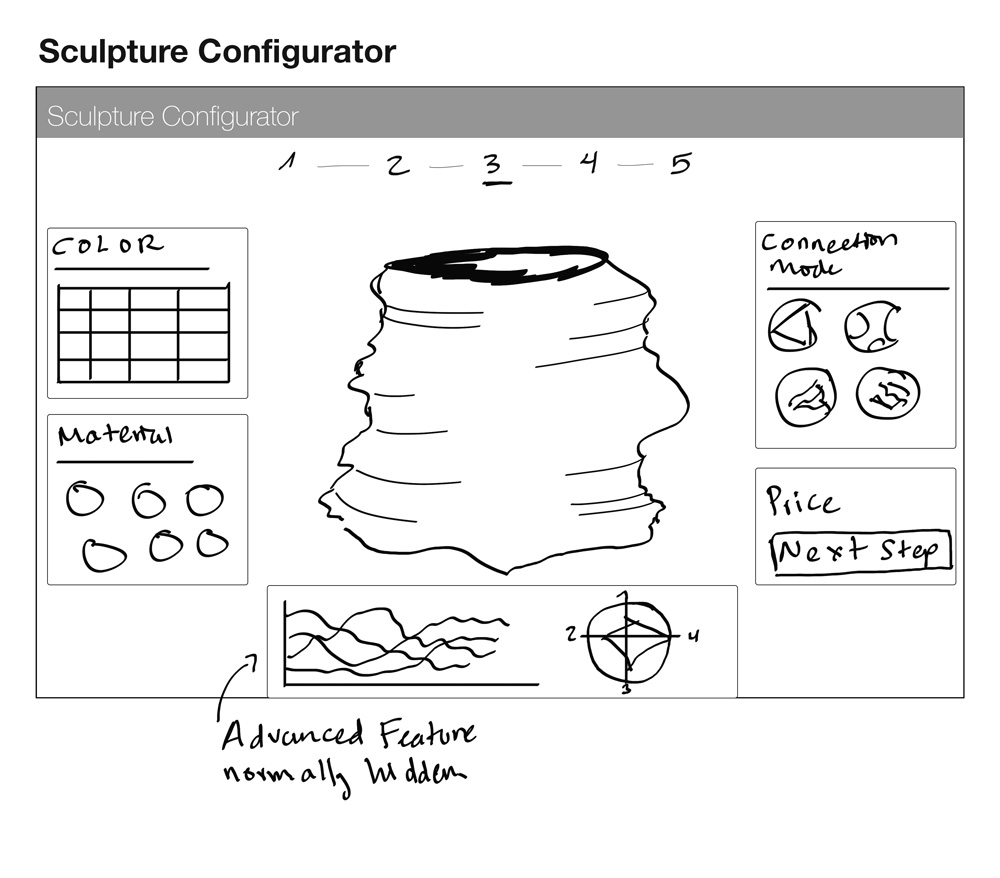
\includegraphics[width=0.6\textwidth,trim=0mm 24mm 0mm 0mm,clip=true]{Prototype/img/ui_proto1}
  \caption{Sketch of the step based configurator prototype}
\label{fig:uiproto1}
\end{center}
\end{figure}

In the second design iteration it was intended to simplify the interface and move from a multi-step based with step-by-step views to a basic multi-step design. The welcome screen first introduced in the first prototype would also remain for all the design iterations. After the user has logged in to the configurator the workspace view is shown. This view contains all the controls for the configurator. In the left side a panel contains several views that can be navigated. Each view has controls for a specific property. The panel shown in figure \ref{fig:uiproto2} has the variable catalog from which the user can chose variables to map to the sculpture. By selecting a variable the sculpture would be instantly updated. The geometry of the sculpture can be customized in another panel with sliders to manipulate height and radius parameters. In this same panel a date field can be used to select the data range of the visualized data.

\begin{figure}[hb]
\centering
\begin{minipage}{.45\textwidth}
\centering
  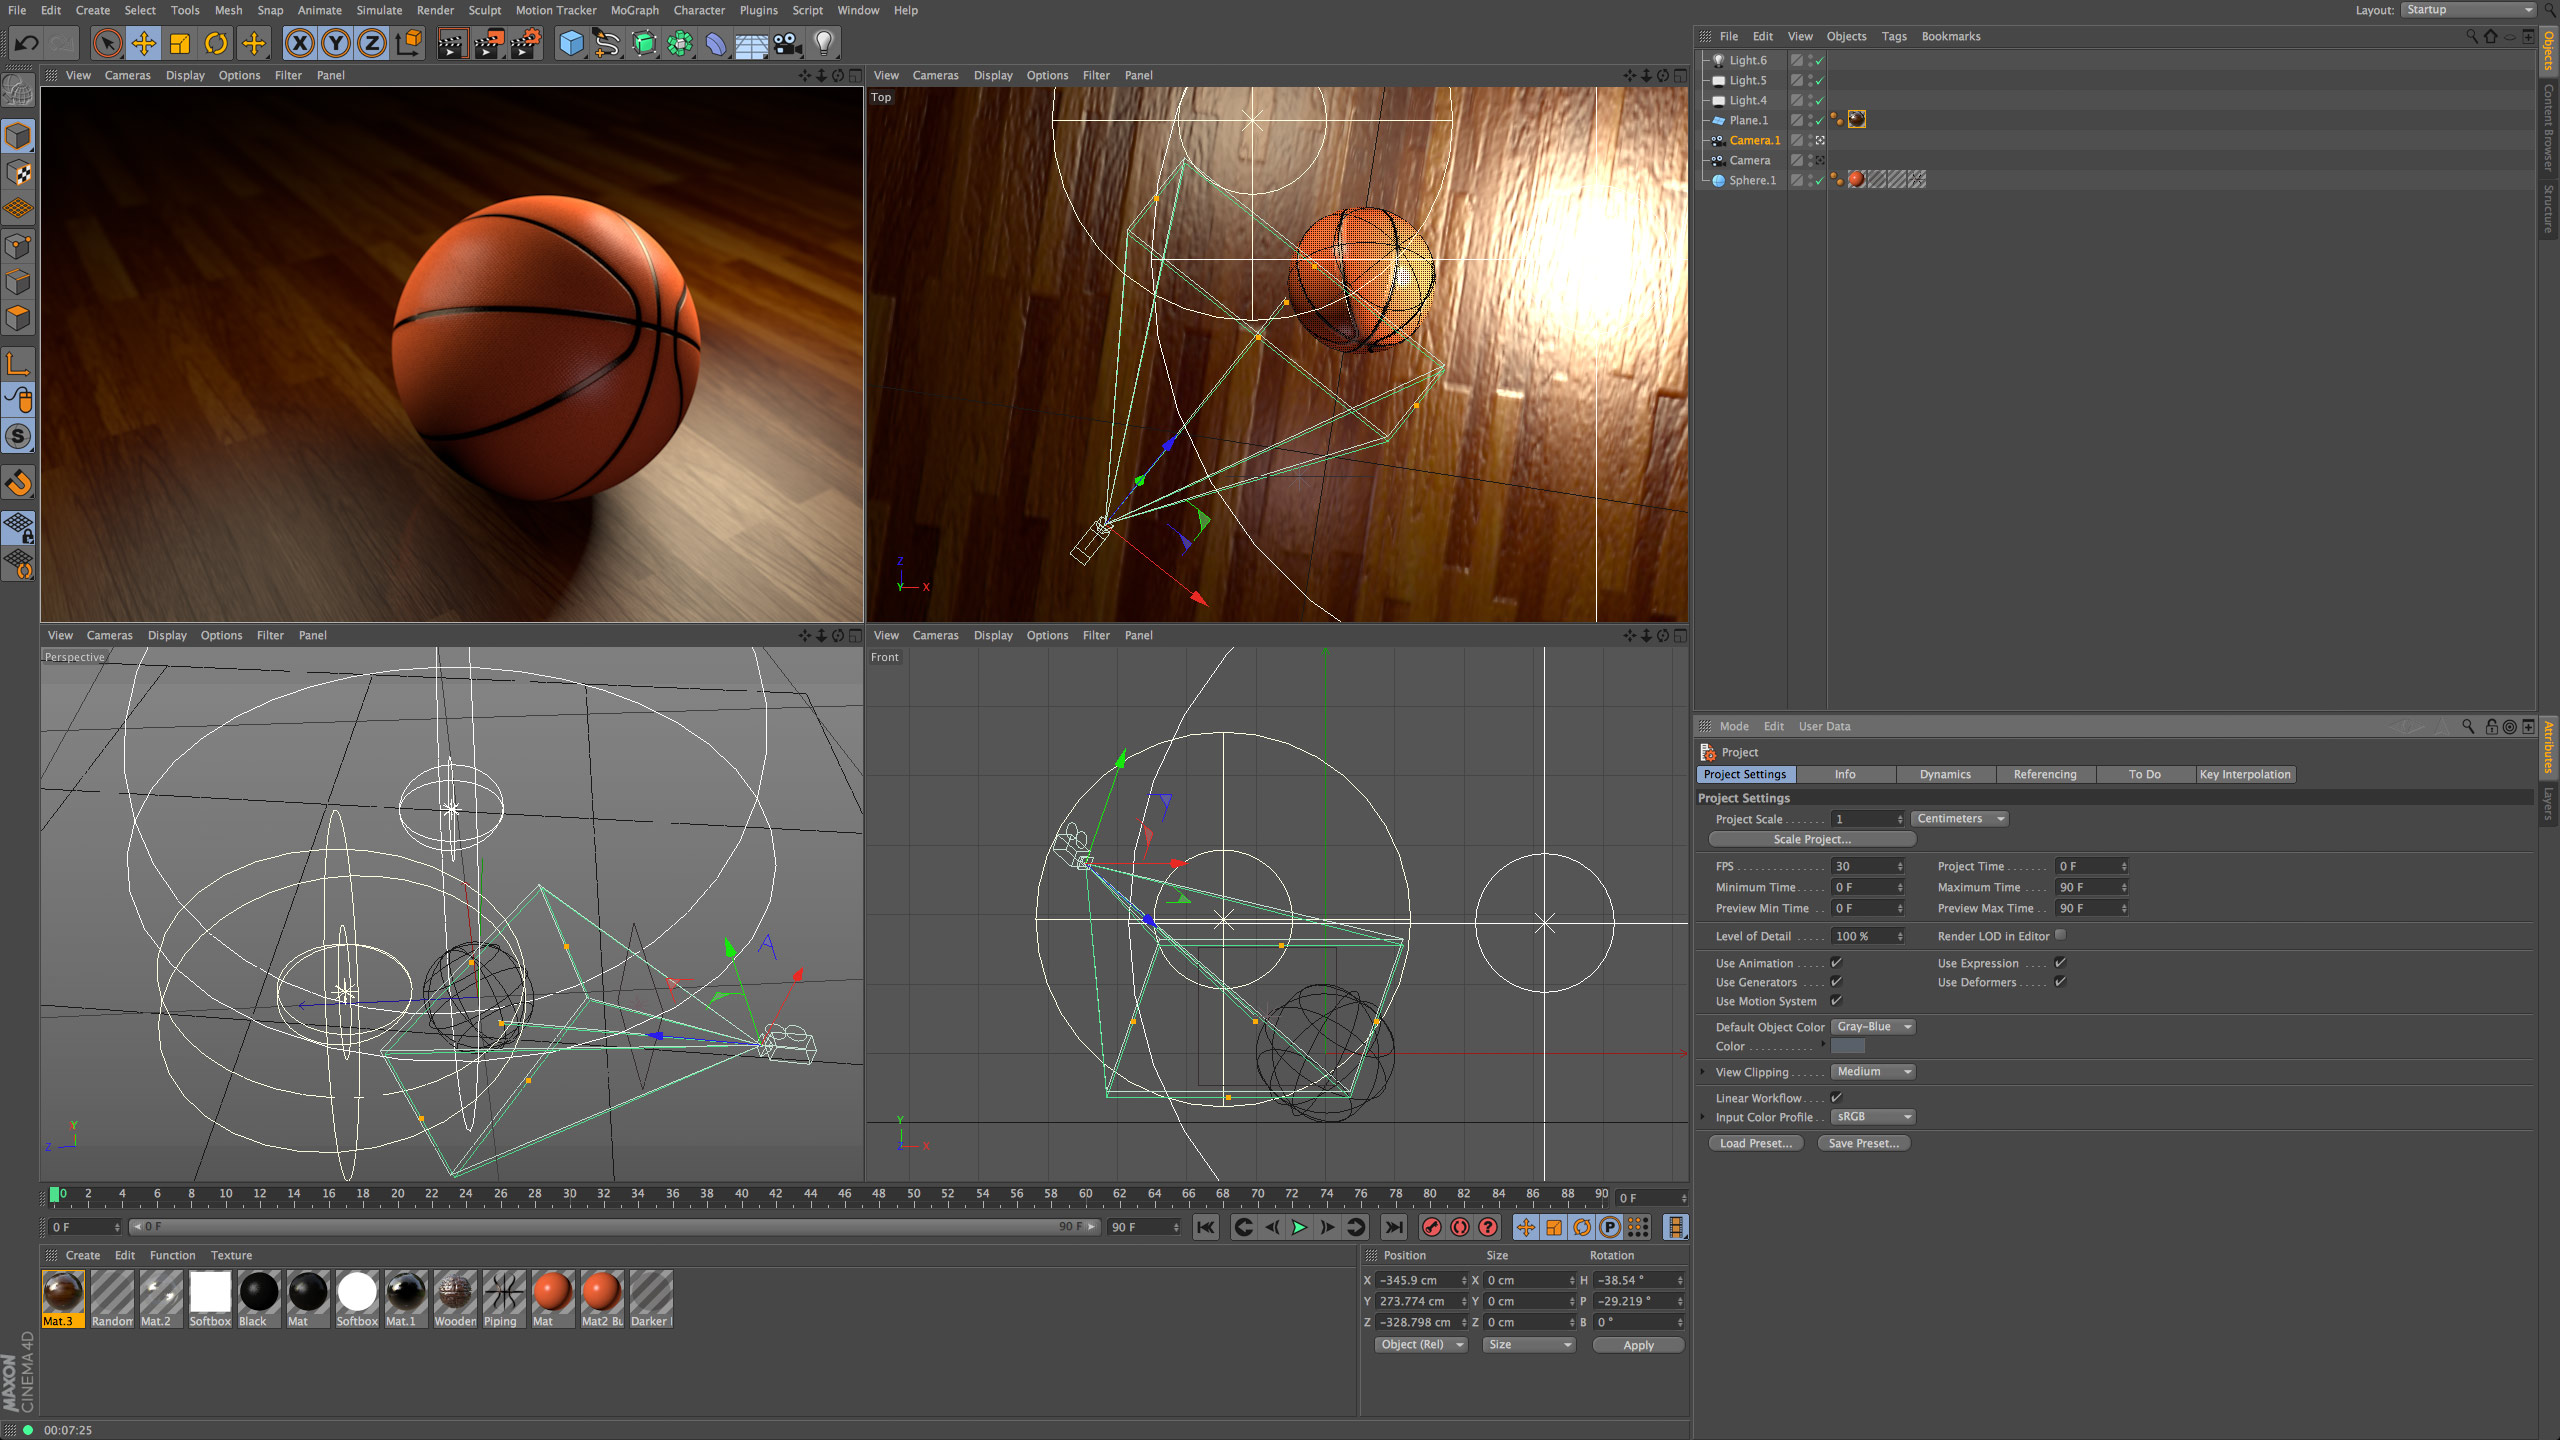
\includegraphics[width=1.06\textwidth,trim=0mm 0mm 50mm 0mm,clip=true]{Prototype/img/cinema4d}
  \caption{3D modeling software Cinema 4D graphical user interface\ \cite{cinema4d}}
  \label{fig:cinema}
\end{minipage}
\begin{minipage}{.45\textwidth}
\centering
  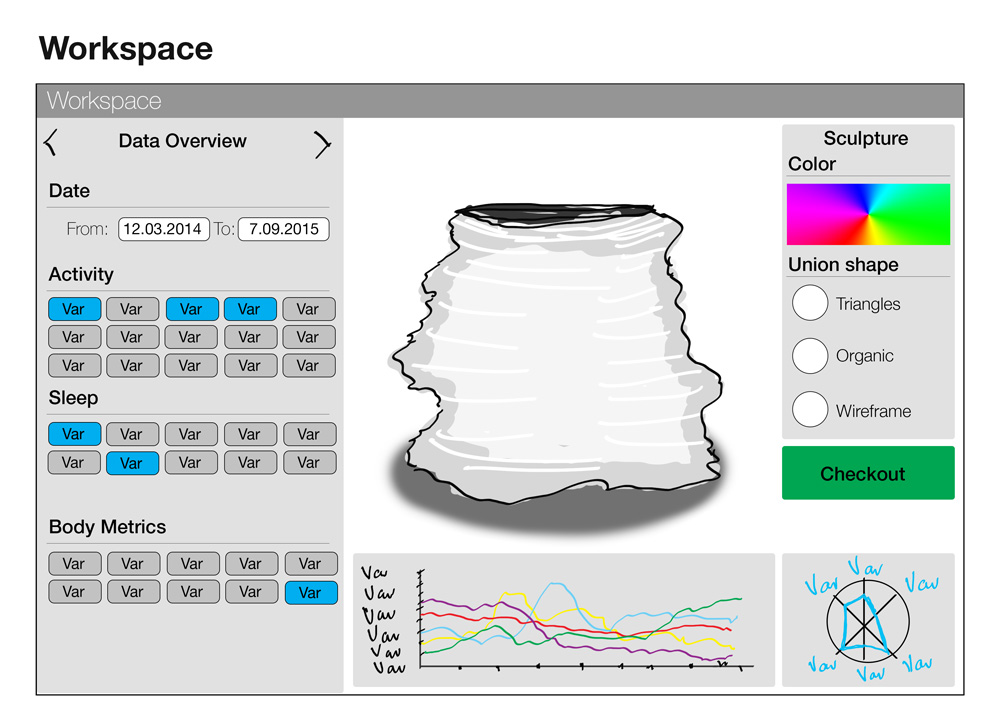
\includegraphics[width=1.0\linewidth,trim=0mm 0mm 0mm 28mm,clip=true]{Prototype/img/ui_proto2}
  \caption{Sketch of 3D modeling software inspired configurator prototype}
  \label{fig:uiproto2}
\end{minipage}
\end{figure}

At the right side a panel with material and color options are shown. Again at the bottom a line- and radial-charts visualize the selected variables. After finishing the user is brought to a summary view of the selected materials and variables visualized. A strong inspiration for this concept were 3D modeling software packages like the one shown in figure \ref{fig:cinema}. The normal layout of modeling software offers users an overview of the scene in different angles and a series of navigation menus and panels with material and assets windows. 

The final design iteration of the configurator was conceived with the goal of further simplify the interface by hiding all panels and instead focus user's attention to the sculpture (see figure \ref{fig:uiproto3}). After logging in the user is taken to the configurator. The sculpture will be surrounded by a circle with floating labels of the selected variables. To edit the visualized variables a button with a plus symbol is placed in the circle around the sculpture. If the user presses this button a panel pop ups displaying the variable list. After selecting a variable the sculpture will update instantly. This prototype has three more buttons. Floating on the right a calendar button can be used to display a slider with which the user can set the data range to be visualized. The other two buttons are used to manipulate geometry and material options. 

In the following section the comparison of the 3 prototypes will be discussed, closing with an argumentation about the chosen prototype. 

\begin{figure}[h]
\captionsetup{width=0.9\textwidth}
\begin{center}
  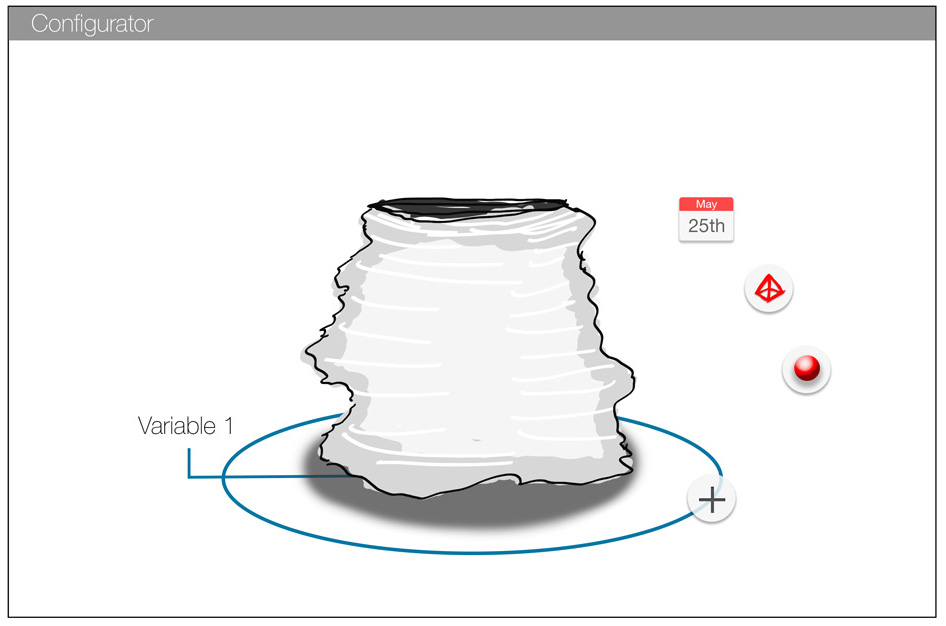
\includegraphics[width=0.6\textwidth]{Prototype/img/ui_proto3}
  \caption{Sketch of a simplified panel-free configurator prototype}
\label{fig:uiproto3}
\end{center}
\end{figure}

\subsubsection{Prototype Validation}
The main difference of the 3 prototypes is how the the user is guided through the configuration process. A welcome view in all prototypes will introduce the worklfow to the user allowing him to get comfortable with the system. The first prototype simplifies the available visual controls by dividing the process in steps. Each step is specialized in a single aspect of the configuration process, this has the benefit of allowing the user to concentrate on a single task an move on. The downside of such an implementation is that it requires state persistence functionality to store the configurations made throughout the process. For the amount of controls available for the activity sculpture configurator this option might be an overkill due that the essential steps can be broken down to two steps. 

On the other hand simplifying the interface so much as in prototype 3 where all controls are accessed through buttons could offers not enough information about how they can achieve their goals. Although this prototype encourages exploration as it is the only way the user can figure out how to customize the sculpture, this takes the configurator to a more sculpting like approach. 

Prototype 2 sits somewhere in the middle between prototype 1 and 3. The step clutter is reduced to a single view but through the display of control panels with text the user has visual queues as to what the available tasks are. Through the left panel that accommodates different controls through a cycling tab system the clutter of customization controls is avoided allowing the user to concentrate in the controls that are visible in the panel at the moment. 

In summary the developed configurator prototype offers a simplified workflow through a basic multi-step approach design with a simple layout that displays the controls in a logically organized manner thanks to a tab panel. The available controls will be reduced to buttons, toggles and sliders that easily configurated in the system and most importantly the user can not make any mistakes, liberating the user of frustrating experiences of correcting mistakes. By having only one view the configurator reduces the implementation complexity and does not require a persistence system.

Chapter \ref{ch:configurator} is devoted to the technical implementation of the configurator's prototype discussing technologies used, the overall architecture and the challenges encountered in the developing process. 

\end{document}